\begin{exercise}{}{exercise_5.1}
    Determine the sample complexity $N(\epsilon, \delta)$ for ERM over a class $\Hf$ with VC dimension $V_\Hf<\infty$.
\end{exercise}

\begin{solution*}[Exercise \ref{ex:exercise_5.1}]
    We have:
    \begin{align*}
        P\bigRound{R(\widehat{h_n}) - R_\Hf^* \ge \epsilon} 
        &\le P\biggRound{
            2\sup_{h\in\Hf}\bigAbs{ \widehat{R_n}(h) - R(h) } \ge \epsilon
        } \\
        &= P\biggRound{
            \sup_{h\in\Hf}\bigAbs{ \widehat{R_n}(h) - R(h) } \ge \frac{\epsilon}{2}
        } \\
        &\le 8S_\Hf(n)e^{-n\epsilon^2/128} \ \ \ (\text{Theorem } \ref{thm:vc_theorem_for_clf}) \\
        &\le 8(n+1)^{V_\Hf} e^{-n\epsilon^2/128} \ \ \ (\text{Corollary } \ref{coro:sauer_bound_on_shattering_coeff_I})
    \end{align*}

    \noindent Now let:
    \begin{align*}
        \delta &= 8(n+1)^{V_\Hf}e^{-n\epsilon^2/128} \\
        \implies
        \log\frac{\delta}{8} &= V_\Hf\log(n+1) - \frac{n\epsilon^2}{128}
        \\
        \implies
        N(\epsilon, \delta) &= \frac{128}{\epsilon^2} \biggRound{
            V_\Hf\log (n+1) - \log\frac{\delta}{8}
        }
    \end{align*}
\end{solution*}

\begin{exercise}{}{exercise_5.2}
    Show that the VC Theorem for sets implies the VC Theorem for classifiers. 

    \noindent\newline\textit{Hint : Consider the sets of the form $G'=G\times\{0\} \cup G^c \times \{1\} \subset \X\times\Y$.}
\end{exercise}

\begin{solution*}[Exercise \ref{ex:exercise_5.2}]
    Given an arbitrary class of classifiers $\Hf$. Define the following class of sets:
    \begin{align*}
        \mathcal{G} = \bigCurl{
            G_h \times \{0\} \cup G_h^c \times \{1\} : h \in \Hf
        }
    \end{align*}

    \noindent Where for a given $h\in\Hf$, we have:
    \begin{align*}
        G_h = \bigCurl{
            x \in \X : h(x) = 1
        }
    \end{align*}

    \noindent Let $P_{XY}$ be the density function over $\X\times\Y$. For any $G\in\mathcal{G}$, we have:
    \begin{align*}
        P_{XY}(G) &= \pi_0P_{X|Y=0}(G) + \pi_1P_{X|Y=1}(G) \\
            &= \pi_0P_{X|Y=0}\Big(G_h \times \{0\} \cup G_h^c \times \{1\}\Big)
                + \pi_1P_{X|Y=1}\Big(G_h \times \{0\} \cup G_h^c \times \{1\}\Big) \\
            &= \pi_0P_{X|Y=0}(G_h) + \pi_1P_{X|Y=1}(G_h^c) \\
            &= \pi_0P_{X|Y=0}(h(X)=1) + \pi_1P(X|Y=1)(h(X)=0) \\
            &= P(h(X) \ne Y) \\
            &= R(h)
    \end{align*}

    \noindent Let $Q=P_{XY}$. We also have:
    \begin{align*}
        \widehat{Q}(G) = \frac{1}{n}\sum_{i=1}^n \1{(X_i, Y_i) \in G_h} = \frac{1}{n}\sum_{i=1}^n \1{h(X_1)\ne Y_i} = \widehat{R_n}(h)
    \end{align*}


    \noindent From the above, we have:
    \begin{align*}
        P\biggRound{
            \sup_{h\in\mathcal{H}} \bigAbs{ \widehat{R_n}(h) - R(h) } \ge \epsilon
        }
        &= P\biggRound{
            \sup_{G\in\mathcal{G}} \bigAbs{ \widehat{Q}(G) - Q(G) } \ge \epsilon
        } \\
        &\le 8S_\mathcal{G}(n)e^{-n\epsilon^2/32} \\
        &=   8S_\mathcal{H}(n)e^{-n\epsilon^2/32} \\
    \end{align*}
\end{solution*}

\begin{exercise}{}{exercise_5.3}
    Let $\G_1$ and $\G_2$ denote two classes of sets:
    \begin{itemize}
        \item ${\bf (a)}$ $\G_1 \cap \G_2=\bigCurl{G_1\cap G_2: G_1\in\G_1, G_2 \in\G_2}$.
        \item ${\bf (b)}$ $\G_1 \cup \G_2=\bigCurl{G_1\cup G_2: G_1\in\G_1, G_2 \in\G_2}$.
    \end{itemize}

    Show that $S_{\G_1\cap\G_2}(n) \le S_{\G_1}(n)S_{\G_2}(n)$ and $S_{\G_1\cup\G_2}(n) \le S_{\G_1}(n)S_{\G_2}(n)$.
\end{exercise}

\begin{solution*}[Exercise \ref{ex:exercise_5.3}]
    Proving each inequality one by one, we have:
    \begin{subproof}{\newline Claim : $S_{\G_1 \cap \G_2}(n) \le S_{\G_1}(n)S_{\G_2}(n)$}
        For any $\{x_1, \dots, x_n\} \subset \X$, denote the following set:

        \begin{align*}
            \F = \bigCurl{
                G_1\cap\{x_1, \dots, x_n\} : G_1 \in \G_1
            }
        \end{align*}

        \noindent Then, $\F$ is a collection of subsets of $\{x_1, \dots, x_n\}$. Furthermore, the cardinality of $\F$ is at most $S_{\G_1}(n)$. Now define the restriction of $\G_1\cap\G_2$ to $\{x_1, \dots, x_n\}$:

        \begin{align*}
            {\G_1 \cap \G_2}_{\{x_1, \dots, x_n \}}
                &= \bigCurl{
                    G_1 \cap G_2 \cap \{ x_1, \dots, x_n \} : G_1 \in \G_1, G_2 \in \G_2
                } \\
                &= \bigcup_{F \in \F} \bigCurl{
                    G_2 \cap F : G_2 \in \G_2
                }
        \end{align*}

        \noindent For each $F\in\F$, we have $|F| \le n$. Hence, we have:
        \begin{align*}
            \bigAbs{\bigCurl{
                G_2 \cap F : G_2 \in \G_2
            }} \le S_{\G_2}(n), \ \forall F \in \F
        \end{align*}

        \noindent Hence,
        \begin{align*}
            \bigAbs{{\G_1 \cap \G_2}_\{x_1, \dots, x_n \}} 
                &= \biggAbs{
                    \bigcup_{F \in \F} \bigCurl{
                        G_2 \cap F : G_2 \in \G_2
                    }
                } \\
                &\le \sum_{F\in\F} \bigAbs{ \bigCurl{
                    G_2 \cap F : G_2 \in \G_2
                }} \\
                &\le \sum_{F\in\F} S_{\G_2}(n) = |\F|S_{\G_2}(n)  \ \ \ (\text{Since } |F| \le n, \forall F\in F)  \\
                &\le S_{\G_1}(n) S_{\G_2}(n)
        \end{align*}

        \noindent Since the above is a uniform bound, we can take the supremum over all $\{x_1, \dots, x_n\}\subset \X$ and the inequality still holds. Hence,
        \begin{align*}
            \sup_{\{ x_1, \dots, x_n \} \subset \X} \bigAbs{
                {\G_1 \cap \G_2}_\{x_1, \dots, x_n \}
            } = S_{\G_1 \cap \G_2}(n) \le S_{\G_1}(n)S_{\G_2}(n)
        \end{align*}
    \end{subproof}

    \begin{subproof}{\newline Claim : $S_{\G_1 \cup \G_2}(n) \le S_{\G_1}(n)S_{\G_2}(n)$}
        For any $\{x_1, \dots, x_n \} \subset \X$, we define the following collections of subsets:
        \begin{align*}
            \F_1 &= \bigCurl{
                G_1 \cap \{ x_1, \dots, x_n \} : G_1 \in \G_1
            } \\
            \F_2 &= \bigCurl{
                G_2 \cap \{ x_2, \dots, x_n \} : G_2 \in \G_2
            }
        \end{align*}

        \noindent Then we have:
        \begin{align*}
            {\G_1 \cup \G_2}_{\{x_1, \dots, x_n \}} 
                &= \bigcup_{F_1 \in \F_1} \bigcup_{F_2\in\F_2} \{ F_1 \cup F_2 \}
        \end{align*}

        \noindent Since $|\F_1| \le S_{\G_1}(n)$ and $|\F_2| \le S_{\G_2}(n)$, we have:
        \begin{align*}
            \bigAbs{{\G_1 \cup \G_2}_{\{x_1, \dots, x_n \}}}
                &= \biggAbs{\bigcup_{F_1 \in \F_1} \bigcup_{F_2\in\F_2} \{ F_1 \cup F_2 \}} \\
                &\le |\F_1||\F_2| \\
                &\le S_{\G_1}(n)S_{\G_2}(n)
        \end{align*}

        \noindent Taking the supremum over $\{x_1, \dots, x_n\}\subset\X$ for both sides, we have:
        \begin{align*}
            \sup_{\{x_1, \dots, x_n\}\subset\X} \bigAbs{{\G_1 \cup \G_2}_{\{x_1, \dots, x_n \}}} = S_{\G_1\cup\G_2}(n) \le S_{\G_1}(n)S_{\G_2}(n)
        \end{align*}
    \end{subproof}
\end{solution*}

\noindent \textbf{Remark} : We can extend the proof for exercise \ref{ex:exercise_5.3} to function classes. Hence, we have the following Corollary for the VC-dimension of ensembled classifiers:

\begin{corollary}{VC-dimension bound for ensembled classifiers}{vc_bound_ensembled_clf}
    Let $\Hf_1$ and $\Hf_2$ be two classes of classifiers and define:
    \begin{itemize}
        \item $(\bf a)$ $\Hf_1\cap\Hf_2 = \bigCurl{ \1{h_1(x)=1 \wedge h_2(x)=1} : h_1 \in \Hf_1, h_2\in\Hf_2 }$.
        \item $(\bf b)$ $\Hf_1\cup\Hf_2 = \bigCurl{ \1{h_1(x)=1 \vee h_2(x)=1} : h_1 \in \Hf_1, h_2\in\Hf_2 }$.
    \end{itemize}

    \noindent We have that $S_{\Hf_1\cap\Hf_2}(n)\le S_{\Hf_1}(n)S_{\Hf_2}(n)$ and $S_{\Hf_1\cup\Hf_2}(n)\le S_{\Hf_1}(n)S_{\Hf_2}(n)$. Furthermore, we have:
    \begin{align*}
        V_{\Hf_1}, V_{\Hf_2} < \infty \implies V_{\Hf_1\cap\Hf_2} < \infty \text{ and } V_{\Hf_1\cup\Hf_2} < \infty
    \end{align*}
\end{corollary}

\begin{proof*}[Corollary \ref{coro:vc_bound_ensembled_clf}]
    The translation of the results in exercise \ref{ex:exercise_5.3} to function classes is trivial. The main point is to prove the second point of the corollary. 
    
    \noindent\newline Assume that the statement does not hold. Hence, $V_{\Hf_1\cap\Hf_2}=\infty$ and $S_{\Hf_1\cap\Hf_2}(n) = 2^n, \forall n\ge1$. By Sauer's lemma \ref{thm:sauer_lemma}, since $V_{\Hf_1}, V_{\Hf_2} < \infty$, we have:
    \begin{align*}
        S_{\Hf_1}(n) &\le (n+1)^{V_{\Hf_1}} \implies \log S_{\Hf_1}(n) \le V_{\Hf_1}\log(n+1) \\
        S_{\Hf_2}(n) &\le (n+1)^{V_{\Hf_2}} \implies \log S_{\Hf_2}(n) \le V_{\Hf_2}\log(n+1)
    \end{align*} 

    \noindent Therefore, we have:
    \begin{align*}
        \log S_{\Hf_1\cap\Hf_2}(n) &\le \log S_{\Hf_1}(n) + \log S_{\Hf_2}(n) \\
        \implies n\log 2 &\le (V_{\Hf_1} + V_{\Hf_2})\log(n+1), \ \forall n\ge1
    \end{align*}

    \noindent However, this is not true since the left-hand-side evolves linearly while the right-hand-side evolves logarithmically. Therefore, we have a contraction $\implies V_{\Hf_1\cap\Hf_2} < \infty$. We can repeat the same argument for $V_{\Hf_1\cup\Hf_2}$.
\end{proof*}


\begin{exercise}{}{exercise_5.4}
    Show that the following classes have finite VC dimension by exhibiting an explicit upperbound on the VC dimension.
    \begin{itemize}
        \item ${\bf (a)}$ $\X=\R^d, \Hf=\{ \1{f(x)\ge0} : f \text{ inhomogeneous quadratic polynomial} \}$.
        \item ${\bf (b)}$ $\X=\R^d, \Hf=\{ \1{x \in C} : C \text{ is a closed sphere }\}$.
        \item ${\bf (c)}$ $\X=\R^2, \Hf=\{ \1{x \in P_k} : P_k \text{ is a convex polygon of at most $k$ sides} \}$.
        \item ${\bf (d)}$ $\X=\R^d, \Hf=\{ \1{x \in R_k} : R_k \text{ is a union of at most $k$ rectangles} \}$.
    \end{itemize}
\end{exercise}

\begin{solution*}[Exercise \ref{ex:exercise_5.4}]
    In the following exercise, we will mostly make use of proposition \ref{prop:steele_dudley} to bound the VC dimension of the above function classes:
    \begin{subproof}{\newline ${\bf (a)}$ $\X=\R^d, \Hf=\{ \1{f(x)\ge0} : f \text{ inhomogeneous quadratic polynomial} \}$}
        Define the following function class of $d$-dimensional inhomogeneous quadratic polynomials:
        \begin{align*}
            \F_1=\bigCurl{
                f:\R^d\to\R \Big| f({\bf x}) = {\bf x^TAx} + {\bf b^Tx} + c, {\bf A} \in \R^{d\times d}, \text{ symmetric}.  \ {\bf b}\in\R^d, c\in\R 
            }
        \end{align*}

        \noindent For any $f\in\F_1$, we can write:
        \begin{align*}
            f({\bf x}) &= \underbrace{\sum_{k=1}^d a_k x_k^2 + 2\sum_{i=1}^d \sum_{j=i+1}^d a_{ij}x_ix_j}_{{\bf x^TAx}} + \underbrace{\sum_{l=1}^d b_l x_l}_{{\bf b^Tx}} + c
        \end{align*}

        \noindent Hence, we have the following basis functions for $\F_1$:
        \begin{align*}
            \mathcal{B} = \bigCurl{
                1, \underbrace{x_1^2, \dots, x_d^2}_{d}, \underbrace{x_1x_2, \dots, x_{d-1}x_d}_{\frac{d(d-1)}{2}}, \underbrace{x_1, \dots, x_d}_{d}
            }
        \end{align*}

        \noindent Therefore, we have:
        \begin{align*}
            \dim(\F_1) = |\mathcal{B}| = \frac{d(d-1)}{2} + 2d + 1
        \end{align*}

        \noindent Therefore, by proposition \ref{prop:steele_dudley}, we have:
        \begin{align*}
            V_\Hf \le \dim(\F_1) = \frac{d(d-1)}{2} + 2d + 1
        \end{align*}
    \end{subproof}

    \begin{subproof}{\newline ${\bf (b)}$ $\X=\R^d, \Hf=\{ \1{x \in C} : C \text{ is a closed sphere }\}$}
        Denote the following function class:
        \begin{align*}
            \F_2 = \biggCurl{
                f:\R^d \to \R \Big| f({\bf x}) = r^2 - \sum_{i=1}^d (x_i - c_i)^2, r\in \R, c_i \in \R
            }    
        \end{align*}
        
        \noindent Where $r$ denotes the radius of the hypersphere and the vector $(c_1, \dots, c_d)^T\in\R^d$ is the coordinates of the center. We can rewrite the class of classifiers as followed:
        \begin{align*}
            \Hf&=\{ \1{x \in C} : C \text{ is a closed sphere }\} \\
            &= \biggCurl{
                \1{f({\bf x}) \ge 0} \Big| f \in \F_2
            }
        \end{align*}

        \noindent We notice that:
        \begin{align*}
            \F_2 \subset \F_1 \implies \dim(\F_2) \le \dim(\F_1)
        \end{align*}

        \noindent Hence, by proposition \ref{prop:steele_dudley}, we have:
        \begin{align*}
            V_\Hf \le \dim(\F_2) \le \dim(\F_1) \le \frac{d(d-1)}{2} + 2d + 1
        \end{align*}
    \end{subproof}

    \begin{subproof}{\newline ${\bf (c)}$ $\X=\R^2, \Hf=\{ \1{x \in P_k} : P_k \text{ is a convex polygon of at most $k$ sides} \}$}
        We can think of $\1{x\in P_k}$ as an ensemble of $k$ different linear classifiers in $\R^2$. This is illustrated in figure \ref{fig:convex_polygon_classifier}.

        \begin{figure}[!ht]
            \centering
            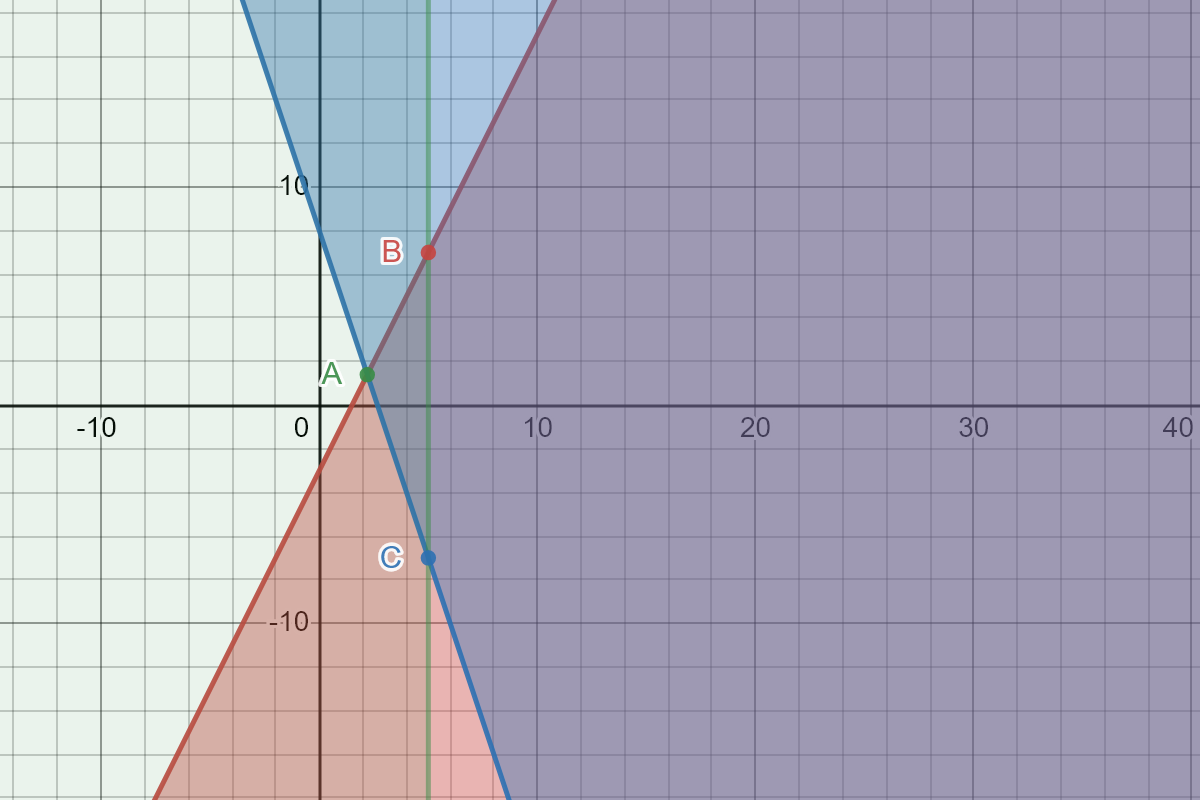
\includegraphics[width=\textwidth]{figures/convex_polygon_classifier.png}
            \caption{Convex polygon comprises of three linear classifiers of the form $\1{f_i(x, y)\ge0}$ where $f_1(x, y) = 2x-y-3$, $f_2(x, y)=3x+y-8$ and $f_3(x, y)=5-x$.}
            \label{fig:convex_polygon_classifier}
        \end{figure}

        \noindent We define the class of linear classifiers in $\R^2$ as followed:
        \begin{align*}
            \mathcal{L} = \bigCurl{
                \1{f(x, y) \ge 0} : f(x, y) = ax + by + c \text{ where } a, b, c \in \R
            }
        \end{align*}

        \noindent Hence, we can rewrite the classifiers class of convex polygons as:
        \begin{align*}
            \Hf
                &=\{ \1{x \in P_k} : P_k \text{ is a convex polygon of at most $k$ sides} \} \\
                &= \biggCurl{
                    \bigwedge_{i=1}^n \1{f_i(x, y) \ge 0} : f_i \in \mathcal{L}, n \le k
                }
        \end{align*}

        \noindent Since $V_\mathcal{L}<\infty$, by corollary \ref{coro:vc_bound_ensembled_clf}, we also have $V_\Hf<\infty$.
    \end{subproof}

    \begin{subproof}{\newline ${\bf (d)}$ $\X=\R^d, \Hf=\{ \1{x \in R_k} : R_k \text{ is a union of at most $k$ rectangles} \}$}
        We can re-define the classifiers class as followed:
        \begin{align*}
            \Hf
                &=\{ \1{x \in R_k} : R_k \text{ is a union of at most $k$ rectangles} \} \\
                &=\biggCurl{\bigvee_{i=1}^n \1{x\in \mathcal{R}_i} : \mathcal{R}_i \text{ is a rectangle }, n\le k}
        \end{align*}
    \end{subproof}

    \noindent Since the class of hyper-rectangles have finite VC-dimension of $2d$, by corollary \ref{coro:vc_bound_ensembled_clf}, we have that $\Hf$ also has finite VC-dimension.
\end{solution*}


